\chapter{Single-Hole Illumination}
\label{ch:singleilluminate}

\texttt{singleilluminate/} provides the unified illumination interface for this
project's single-hole case (its multi-hole array extension is explicitly out of scope
for this report --- see Chapter~\ref{ch:introduction}). It reuses
Equation~\eqref{eq:erel} directly, cross-checked at import time against
\texttt{photometry.py}'s independently-implemented version of the same formula (both
must agree to $10^{-12}$ relative tolerance, checked automatically, or the module
refuses to run) --- a real, executable consistency check between two independently
written implementations of the same physical relationship, not merely a documented
claim that they agree.

\begin{figure}[htbp]
\centering
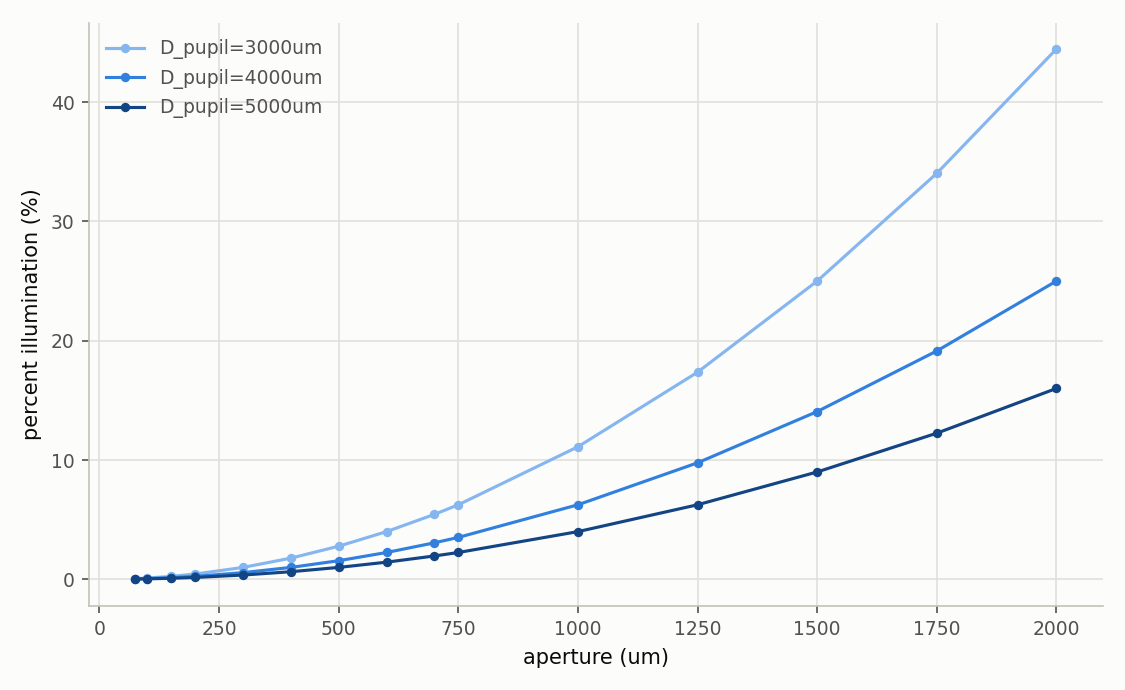
\includegraphics[width=0.85\textwidth]{figures/fig_singleilluminate.png}
\caption{Percent illumination vs.\ aperture, for three natural pupil diameters (3, 4, 5\,mm).}
\label{fig:singleilluminate}
\end{figure}

{\small
\begin{longtable}{rrr}
\caption{Single-hole percent illumination vs. aperture and natural pupil diameter.}\label{tab:singleilluminate-full}\\
\toprule
a\_hole (um) & D\_pupil (um) & percent illumination (\%) \\
\midrule
\endfirsthead
\multicolumn{3}{c}{\tablename\ \thetable\ -- continued}\\
\toprule
a\_hole (um) & D\_pupil (um) & percent illumination (\%) \\
\midrule
\endhead
\bottomrule
\endfoot
75.000 & 3000.000 & 0.062 \\
100.000 & 3000.000 & 0.111 \\
150.000 & 3000.000 & 0.250 \\
200.000 & 3000.000 & 0.444 \\
300.000 & 3000.000 & 1.000 \\
400.000 & 3000.000 & 1.778 \\
500.000 & 3000.000 & 2.778 \\
600.000 & 3000.000 & 4.000 \\
700.000 & 3000.000 & 5.444 \\
750.000 & 3000.000 & 6.250 \\
1000.000 & 3000.000 & 11.111 \\
1250.000 & 3000.000 & 17.361 \\
1500.000 & 3000.000 & 25.000 \\
1750.000 & 3000.000 & 34.028 \\
2000.000 & 3000.000 & 44.444 \\
75.000 & 4000.000 & 0.035 \\
100.000 & 4000.000 & 0.062 \\
150.000 & 4000.000 & 0.141 \\
200.000 & 4000.000 & 0.250 \\
300.000 & 4000.000 & 0.562 \\
400.000 & 4000.000 & 1.000 \\
500.000 & 4000.000 & 1.562 \\
600.000 & 4000.000 & 2.250 \\
700.000 & 4000.000 & 3.062 \\
750.000 & 4000.000 & 3.516 \\
1000.000 & 4000.000 & 6.250 \\
1250.000 & 4000.000 & 9.766 \\
1500.000 & 4000.000 & 14.062 \\
1750.000 & 4000.000 & 19.141 \\
2000.000 & 4000.000 & 25.000 \\
75.000 & 5000.000 & 0.022 \\
100.000 & 5000.000 & 0.040 \\
150.000 & 5000.000 & 0.090 \\
200.000 & 5000.000 & 0.160 \\
300.000 & 5000.000 & 0.360 \\
400.000 & 5000.000 & 0.640 \\
500.000 & 5000.000 & 1.000 \\
600.000 & 5000.000 & 1.440 \\
700.000 & 5000.000 & 1.960 \\
750.000 & 5000.000 & 2.250 \\
1000.000 & 5000.000 & 4.000 \\
1250.000 & 5000.000 & 6.250 \\
1500.000 & 5000.000 & 9.000 \\
1750.000 & 5000.000 & 12.250 \\
2000.000 & 5000.000 & 16.000 \\
\end{longtable}
}

As expected from Equation~\eqref{eq:erel}, percent illumination grows quadratically
with aperture up to $a_{hole}=D_{pupil}$ and saturates at $100\%$ beyond it; a larger
natural pupil shifts the saturation point outward and lowers percent illumination at
any fixed aperture below it, since the same physical aperture area represents a
smaller fraction of a larger pupil's area.
